% =============================================================
%  chch-robot 学术论文：面向中国象棋的人机对弈机器人系统
%  编译：xelatex + biber + xelatex + xelatex
%  字体：ctex 默认 Windows 字体集（宋体/黑体/仿宋/楷体）
%  文档类：ctexbook（每章独立分页）
% =============================================================
\documentclass[UTF8, a4paper, 11pt, openany]{ctexbook}

% ---------- 版面与基础宏包 ----------
\usepackage[margin=2.5cm, headheight=14pt]{geometry}
\usepackage{amsmath, amssymb}
\usepackage{graphicx}
\usepackage{booktabs}
\usepackage{xcolor}
\usepackage{enumitem}
\usepackage{tikz}
\usetikzlibrary{positioning, arrows.meta, fit, calc, shapes.geometric, shadows}
\usepackage{adjustbox}      % 防止图/表超出纸张：max width 约束
\usepackage{tabularx}       % 宽表自动换行
\usepackage{float}

% 允许在 \texttt 的下划线处断行，避免长标识符溢出右边界
\renewcommand{\_}{\textunderscore\allowbreak}
\setlength{\emergencystretch}{4em}

% ---------- 超链接（含中文书签） ----------
\usepackage{hyperref}
\hypersetup{
  colorlinks=true,
  linkcolor=blue,
  citecolor=blue,
  urlcolor=blue,
  pdfencoding=auto,
  pdftitle={面向中国象棋的人机对弈机器人系统设计与实现},
  pdfauthor={Maicarons}
}

% ---------- 参考文献（GB/T 7714-2015） ----------
\usepackage{xstring}
\usepackage[backend=biber, style=gb7714-2015]{biblatex}
\addbibresource{chch-robot-paper.bib}
% 兼容修复：部分 biblatex 版本下 gb7714-2015 的 \multinumberparser
% 依赖 xstring 的赋值未生效，导致 \multinumberfirst 未定义；此处重写为不依赖 xstring 的稳健版本。
\providecommand{\multinumberfirst}{}
\providecommand{\multinumbersecond}{}
\renewcommand{\multinumberparser}[1]{\def\multinumberfirst{#1}\def\multinumbersecond{}}

% ---------- 让每一章直接落在下一页（不插空白页） ----------
\let\cleardoublepage\clearpage

% ---------- 正文开始 ----------
\title{面向中国象棋的人机对弈机器人系统设计与实现\\
\large ——基于视觉识别、Pikafish 引擎与 STM32 运动控制}
\author{Maicarons}
\date{2026 年 8 月}

\begin{document}
\maketitle

% ============================================================
\chapter*{摘\quad 要}
中国象棋（Xiangqi）是世界上参与人数最多的棋类运动之一，其人机对弈长期以来依赖纯软件引擎：
引擎在屏幕上输出着法，由人类完成物理落子。将“感知—决策—执行”三者闭环到一台物理机器人上，
需要同时解决视觉棋盘识别、棋局智能决策与机械臂精确移子等跨学科难题，是具身智能
（embodied AI）在棋类场景中的典型体现。

本文系统介绍 CH-RO（Chinese Chess Robot）对弈机器人系统：一套以 Python 服务、Web 操作界面、
UCI 中国象棋引擎与 STM32 下位机固件构成的完整闭环。在感知层，系统首先建立摄像机针孔成像模型，
采用 RTMPose 四角关键点检测与透视变换完成棋盘定位，并以单一全局分类器 ONNX 模型一次性输出
整盘 $90$ 个交叉点的类别（14 种棋子 + 空 + 未识别），避免了逐格检测与目标检测器的调度与后处理开销；
多帧稳定投票与基于象棋规则的动态走子推断进一步提升了鲁棒性。在认知层，系统通过 UCI 协议驱动
Pikafish 引擎（UCI\_Variant 设为 xiangqi），并以扩展 FEN 表示棋局状态；本文对 alpha-beta 剪枝、
迭代加深与 NNUE 神经评估等搜索原理作了说明。在执行层，系统定义了一种仅含五个整数的 ASCII 指令
协议（startX, startY, endX, endY, signal），经 TCP 端口 8086 下发至 STM32，由下位机完成 SCARA
逆运动学解算与气泵抓取；完成确认以 “STATE:5, RESULT:1” 握手实现。接口层基于 Flask 提供实时视频、
单步/连续识别、硬件与仿真双模式对弈的人机交互。论文给出系统模块划分、识别流水线、协议字段与
坐标映射公式，并以真实代码规模与测试覆盖数据说明工程实现与质量保障。整套系统在解耦、可测试的
代码架构下运行，可为象棋机器人及类似的“视觉—决策—执行”具身智能系统提供参考。

\paragraph{关键词} 中国象棋；人机对弈；机器人；视觉识别；RTMPose；UCI 协议；Pikafish；NNUE；STM32；ONNX

\clearpage
\tableofcontents
\clearpage
\listoffigures
\listoftables
\clearpage

% ============================================================
\chapter{绪\quad 论}
\label{ch:intro}

\section{研究背景与意义}
中国象棋是一种在 $9$ 列 $\times$ $10$ 行交叉点棋盘上进行的两人对弈棋类游戏，棋盘中央以“河界”
分隔双方领地，并在两端设有“九宫”等规则约束\cite{xiangqi2024}。作为与西洋棋并列的最具影响力的
棋类之一，计算机中国象棋历经数十年发展，已出现以象眼（ElephantEye）、Pikafish 等为代表的强引擎；
其中 Pikafish 是从 Stockfish 派生、面向中国象棋的免费开源 UCI 引擎，采用 NNUE 神经评估函数，
是当前最强的开源中国象棋引擎之一\cite{pikafish2024,stockfish2024}。然而，绝大多数相关研究停留在
纯软件层面：引擎在屏幕上输出着法，由人类落子。将决策结果转化为物理世界中的真实移子动作，需要
构建“摄像头识别棋盘—引擎决策—机械臂执行”的闭环系统，这正是具身智能在棋类场景中的典型体现，
对服务机器人、教育机器人与人机协作均有借鉴意义。

\section{国内外研究现状}
\label{sec:related}
计算机棋类博弈是人工智能的经典试验场。在西洋棋方向，深蓝（Deep Blue）于 1997 年首次在标准时限下
战胜国际象棋世界冠军，其基于大规模并行硬件与手工评估函数的搜索体系奠定了后续工程范式
\cite{campbell2002deepblue}；而强化学习方法的引入则进一步改变了范式——TD-Gammon 用时序差分学习
直接从自我对弈中习得西洋棋后端博弈策略\cite{tesauro1995tdgammon}，KnightCap 将 TD($\lambda$) 与
博弈树搜索结合提升棋力\cite{baxter1998knightcap}，直至 AlphaZero 以通用强化学习算法在自我对弈中
同时掌握国际象棋、将棋与围棋，展示了“搜索 + 深度表征”的通用性\cite{silver2018mastering}。在
算法层面，alpha-beta 剪枝、迭代加深与静态搜索（quiescence search）仍是现代引擎的基石，并在
《人工智能：一种现代方法》等教材中有系统论述\cite{russell2020ai}。

在引擎接口层面，通用国际象棋接口 UCI（Universal Chess Interface）由 Meyer-Kahlen 等人于 2004 年
规范，以标准输入/输出文本指令通信\cite{uci2004}；中国象棋则有借鉴 UCI 的 UCCI（Universal Chinese
Chess Interface）协议\cite{ucci2007} 与扩展棋局表示 XQFEN\cite{xqfen2007}，使不同引擎可在统一协议
下被调用。Pikafish 在实现上复用 UCI 框架，并通过 UCI\_Variant 选项支持中国象棋变体\cite{pikafish2024}。
自 2018 年 Nasu 提出 NNUE（Efficiently Updatable Neural-Network-based Evaluation）以来，神经评估
逐渐取代手工评估，成为开源引擎的主流\cite{nasu2018nnue}。

在视觉感知层面，棋类棋盘识别经历了从传统方法到深度学习的演进。早期工作依赖棋盘纹理的规则性，
使用 OpenCV 的 \texttt{findChessboardCorners} 检测内角点完成定位\cite{bradski2000opencv}；但中国象棋
棋盘存在文字棋子遮挡、纹理不完整等问题，纯角点法鲁棒性不足。近年来，基于关键点的方案展现出优势：
RTMPose 是 OpenMMLab MMPose 提出的实时多人姿态估计框架，在 COCO 上以 90+ FPS 取得 75.8\% AP，
可在移动端部署\cite{jiang2023rtmpose,mmpose2023}；其底层采用 SimCC（Simple Coordinate Classification）
关键点范式，用“坐标分类”替代高斯热图回归，实现高精度与低延迟\cite{li2022simcc}，非常契合约束
场景下的棋盘四角定位。在棋子识别上，通用目标检测器（如 YOLO\cite{redmon2016yolo}）虽通用，但逐子
检测存在调度与后处理开销；而受 ImageNet 预训练与深度卷积网络（AlexNet\cite{krizhevsky2012alexnet}、
ImageNet\cite{deng2009imagenet}）启发的“整盘一次性分类”思路，则更适合边缘部署。模型部署侧，ONNX
提供了开放的神经网络交换格式\cite{onnx2019}，ONNX Runtime 则提供跨平台、支持 CUDA/DML/CPU 多种
执行提供者的高性能推理后端\cite{onnxruntime2024}，便于将训练好的模型部署到异构硬件。

在机械执行层面，棋类机器人早期以西洋棋机械臂为主，核心难点在于棋子抓取规划与视觉定位。SCARA
等平面关节机器人的运动学建模与控制已有成熟教材体系\cite{craig2017robotics,siciliano2016handbook}，
而 STM32 等低成本微控制器凭借丰富的定时器与通信外设，常作为下位机承担逆解与电机/气泵时序
\cite{stm32f103}。本文工作正是在上述“强引擎 + 关键点视觉 + 边缘推理 + 低成本下位机”的技术
成熟度基础上，构建一套完整、可解耦、可测试的中国象棋对弈机器人。

\section{问题与挑战}
将软件博弈闭环到物理机器人，面临三方面挑战：
\begin{enumerate}[label=(\arabic*)]
  \item \textbf{视觉识别的鲁棒性}：真实桌面存在光照变化、棋子文字遮挡、视角倾斜与镜头畸变，
        需在边缘算力下以低延迟输出准确棋局。
  \item \textbf{决策与物理执行的对齐}：引擎输出的是逻辑着法（UCI 坐标），必须精确映射到机械臂
        坐标系并安全执行；任何坐标错配都会导致抓错子或碰子。
  \item \textbf{系统可维护性与可测试性}：视觉、决策、控制三者耦合度高，若缺乏清晰的数据契约与
        解耦架构，难以独立调试与回归测试。
\end{enumerate}

\section{研究目标与主要贡献}
本文目标是给出一套\textbf{可解耦、可测试、可联调}的中国象棋对弈机器人完整实现，并就其关键设计
给出严谨描述。主要贡献如下：
\begin{enumerate}[label=(\arabic*)]
  \item 提出“感知—认知—执行—接口”四层系统架构，并以纯函数工具包、命令行包、Web 组合根等方式
        实现模块解耦（模块规模见表~\ref{tab:scale}），使视觉、决策、控制可独立测试。
  \item 设计轻量棋盘识别方案：建立摄像机针孔模型，以 RTMPose 四角关键点完成透视校正，再以单一
        全局分类器一次性输出全棋盘 $90$ 个交叉点类别，避免逐格检测与目标检测器的推理开销。
  \item 定义并实现一种仅含五个整数的 ASCII 五值指令协议与持久化 TCP 客户端，配合 STM32 下位机的
        运动学解算与“STATE:5, RESULT:1”完成确认握手，保证走子的确定性。
  \item 提供硬件/仿真双模式与基于 Flask 的 Web 操作界面，使系统在无实体机械臂时亦可完成端到端联调。
\end{enumerate}

\section{论文结构}
第~\ref{ch:arch} 章给出系统总体架构；第~\ref{ch:vision} 章详述视觉识别流水线及其数学原理；
第~\ref{ch:ai} 章介绍决策引擎、搜索原理与棋局表示；第~\ref{ch:robot} 章阐述机械臂控制协议、
坐标映射、TCP 握手与固件实现；第~\ref{ch:web} 章说明软件编排与 Web 仿真；第~\ref{ch:eng} 章给出
工程实现与质量保障数据；第~\ref{ch:exp} 章汇总真实系统指标；第~\ref{ch:disc} 章讨论设计权衡与局限；
第~\ref{ch:conc} 章总结并展望未来工作。

% ============================================================
\chapter{系统总体架构}
\label{ch:arch}
CH-RO 系统由感知、认知、执行与接口四个层次构成，各层之间仅通过明确的数据契约（图像帧、FEN 字符串、
五值指令、ACK 报文）耦合，从而支持独立替换与测试。整体架构如图~\ref{fig:arch} 所示。

\begin{figure}[H]
\centering
\adjustbox{max width=\textwidth}{%
\begin{tikzpicture}[
    layer/.style={rectangle, draw, rounded corners, minimum width=13cm, minimum height=1.0cm,
                  align=center, font=\small\bfseries, fill=#1!12},
    arrow/.style={-{Latex[length=2.5mm]}, thick, blue!60!black},
    iface/.style={rectangle, draw, dashed, minimum width=13cm, minimum height=0.9cm,
                  align=center, font=\small, fill=gray!10}
  ]
  \node[layer=red]    (p)  {感知层\\摄像头采集 \quad·\quad RTMPose 四角定位 \quad·\quad 全局分类器 \quad·\quad 多帧稳定};
  \node[layer=orange,below=0.4cm of p] (c) {认知层\\Pikafish UCI 引擎 \quad·\quad FEN 棋局状态 \quad·\quad 走法决策};
  \node[layer=teal, below=0.4cm of c] (a) {执行层\\五值协议客户端 \quad·\quad STM32 固件 \quad·\quad SCARA 逆解 \quad·\quad 机械臂};
  \node[iface, below=0.4cm of a] (i) {接口层（Flask Web, 端口 5000）：实时视频 · 单步/连续识别 · 硬件/仿真双模式 · 人机交互};
  \draw[arrow] (p) -- (c);
  \draw[arrow] (c) -- (a);
  \draw[arrow] (a) -- (i);
  \draw[arrow] (i.east) to[out=0, in=0, distance=1.0cm] node[right, font=\tiny, blue!60!black] {状态/视频回传} (p.east);
\end{tikzpicture}}
\caption{CH-RO 系统四层架构。感知层将物理棋盘转为 FEN；认知层生成走法；执行层驱动机械臂；
接口层以 Web 方式贯穿各层并提供人机交互。}
\label{fig:arch}
\end{figure}

\section{四层架构与数据契约}
\begin{itemize}[itemsep=2pt]
  \item \textbf{感知层}：输入为图像帧，输出为 FEN 字符串。其职责是“看见棋盘”。
  \item \textbf{认知层}：输入为 FEN，输出为 UCI 着法（如 \texttt{h2e2}）。其职责是“想出下一步”。
  \item \textbf{执行层}：输入为 UCI 着法，输出为五值指令与机械臂动作，并最终以 ACK 报文确认完成。
  \item \textbf{接口层}：横向贯穿三层，提供人机交互、状态可视与模式切换。
\end{itemize}
四层之间不共享可变全局状态（除 Web 组合根持有受控的共享字典外），而是通过纯函数（FEN 解析、
坐标映射）与消息（五值指令、ACK）通信，这是系统可测试性的根本来源。

\section{模块职责与解耦策略}
系统的主要 Python 包及其职责如表~\ref{tab:modules} 所示。其中 \texttt{xq\_utils} 是由原根目录
\texttt{utils.py} 拆分出的纯函数包，集中实现 FEN、坐标与记谱工具；\texttt{web\_simulation} 以组合根
（composition root）加蓝图（Blueprint）的方式组织 Flask 应用，是当前激活的硬件控制路径。

\begin{table}[H]
\centering
\caption{系统主要模块及其职责}
\label{tab:modules}
\renewcommand{\arraystretch}{1.25}
\begin{tabularx}{\textwidth}{@{}>{\ttfamily\small}l >{\ttfamily\small}X X@{}}
\toprule
模块 & 关键类/函数 & 职责 \\
\midrule
\texttt{xq\_utils} & FENUtils, CoordinateUtils, MoveNotationUtils, BoardUtils & 中国象棋 FEN 解析/生成、棋盘坐标与 UCI 互转、简化 WXF/中文记谱 \\
\texttt{vision} & BoardRecognizer, CameraManager, ChessboardDetector & 摄像头采集、棋盘定位、整盘识别、多帧稳定与动态走子推断 \\
\texttt{core} & ChessboardDetector(ONNX) & RTMPose 四角关键点与全局分类器的推理核心 \\
\texttt{ai} & AIEngine & Pikafish UCI 引擎封装（position/go/bestmove） \\
\texttt{robot} & RobotPersistentClient, uci\_to\_arm\_command & 五值指令协议、持久化 TCP 客户端、UCI 到机械臂指令映射 \\
\texttt{game\_manager} & GameManager & 无界面（仿真）对弈主循环编排 \\
\texttt{web\_simulation} & app, domain, robot\_cmd, game\_logic & Flask 组合根、纯棋局函数、机器人指令封装、状态机与路由 \\
\texttt{config.py} & 模块级常量 & 摄像头、棋盘、引擎、机器人网络与标定的集中配置 \\
\bottomrule
\end{tabularx}
\end{table}

% ============================================================
\chapter{视觉感知与棋盘识别}
\label{ch:vision}
视觉子系统负责把“一张桌子上的物理棋盘”转换为机器可读的 FEN 字符串。其流水线如图~\ref{fig:pipeline}
所示，包含图像采集、棋盘定位、整盘分类、FEN 生成与多帧稳定五个阶段。

\begin{figure}[H]
\centering
\adjustbox{max width=\textwidth}{%
\begin{tikzpicture}[
    node/.style={rectangle, draw, rounded corners, minimum height=1cm, minimum width=2.3cm,
                 align=center, font=\small, fill=blue!8},
    arr/.style={-{Latex[length=2.2mm]}, thick}
  ]
  \node[node] (img)  {原始图像\\(USB / 网络 MJPEG)};
  \node[node, right=0.35cm of img]  (kp)  {四角关键点\\RTMPose};
  \node[node, right=0.35cm of kp]   (warp){透视变换\\450$\times$500};
  \node[node, right=0.35cm of warp] (cls) {全局分类\\90$\times$16};
  \node[node, right=0.35cm of cls]  (fen) {FEN 生成};
  \node[node, below=0.6cm of cls, fill=orange!12] (stab){多帧稳定 \&\\动态走子推断};
  \draw[arr] (img) -- (kp) -- (warp) -- (cls) -- (fen);
  \draw[arr] (cls) -- (stab);
  \draw[arr] (stab.west) to[out=180, in=270, distance=0.8cm] (warp.south);
\end{tikzpicture}}
\caption{视觉识别流水线：从原始图像经四角关键点定位、透视校正，到全局分类与 FEN 生成，
再由多帧稳定模块对连续帧去噪并推断人类走子。}
\label{fig:pipeline}
\end{figure}

\section{图像采集与摄像机模型}
\label{sec:camera}
系统支持两类图像来源：本地 USB 摄像头（通过 OpenCV \texttt{VideoCapture} 采集）与网络摄像头
（如 Orange Pi / Raspberry Pi 提供的 MJPEG 快照或流，由 \texttt{HttpSnapshotCapture} 拉取）\cite{bradski2000opencv}。
采集参数由 \texttt{config.py} 集中配置：分辨率 $640\times480$、帧率 $30$~FPS、设备索引 1，并可在
启动时通过 \texttt{startup.py} 覆盖。

从几何上看，摄像头成像可建模为针孔模型：三维世界点 $\mathbf{X}=[X,Y,Z]^{\top}$ 经投影矩阵
$\mathbf{P}$ 映射到图像像素 $\mathbf{x}\sim\mathbf{P}\mathbf{X}$。当摄像头近似垂直俯视棋盘时，
棋盘平面与像平面近似为一般位置的两平面，其间的映射可统一用一个 $3\times3$ 单应矩阵
（homography）$\mathbf{H}$ 描述（详见下一节）。这一建模是透视校正的理论基础\cite{hartley2004mvp}。

\section{棋盘定位：四角关键点与透视变换}
\label{sec:locate}
与依赖规则棋盘纹理的 \texttt{findChessboardCorners} 不同，本系统使用一个定制 RTMPose ONNX 模型，
直接预测棋盘的\textbf{四个角点}（记为 A0、A8、J0、J8，分别对应左上、右上、左下、右下交叉点）\cite{jiang2023rtmpose,li2022simcc}。
四点经有效性门限（形状为 $(4,2)$、四角置信度均不低于 $0.20$、边距容差 $80$ 像素）校验后，通过
单应矩阵将原始图像校正为归一化俯视图。

\subsection{单应矩阵与透视校正原理}
设棋盘平面上的源点 $\mathbf{x}_s=(u_s,v_s,1)^{\top}$ 与俯视图上的目标点
$\mathbf{x}_d=(u_d,v_d,1)^{\top}$ 满足
\begin{equation}
\label{eq:homo}
\lambda \mathbf{x}_d = \mathbf{H}\,\mathbf{x}_s,\qquad
\mathbf{H}=
\begin{bmatrix}
h_{11} & h_{12} & h_{13}\\
h_{21} & h_{22} & h_{23}\\
h_{31} & h_{32} & h_{33}
\end{bmatrix},
\end{equation}
其中 $\lambda$ 为尺度因子，$\mathbf{H}$ 含 $8$ 个自由度（在归一化 $h_{33}=1$ 下）。已知四对对应点
即可列出 $8$ 个线性方程唯一求解 $\mathbf{H}$。系统调用 OpenCV 的 \texttt{getPerspectiveTransform}
完成该求解，并将原始图像以 \texttt{warpPerspective} 校正为 $450\times500$ 像素的俯视图（即每列 $50$
像素、每行 $50$ 像素）\cite{hartley2004mvp}。由于姿态模型推理开销较大，系统对关键点结果进行缓存
（默认刷新间隔 $8.0$~s 或最多 $120$ 帧），在不移动摄像头的前提下避免每帧重算。

\section{整盘棋子分类}
\label{sec:classify}
校正后的整张棋盘图像被\textbf{一次性}送入一个全局分类器 ONNX 模型，输出形状为 $90\times16$ 的张量，
即 $10$ 行 $\times$ $9$ 列共 $90$ 个交叉点，每个点对应一个 $16$ 维 softmax。这 $16$ 个类别包含
“空”（\texttt{.}）、“未识别”（\texttt{x}）以及红黑双方的 $14$ 种棋子，具体映射如表~\ref{tab:classes}
所示。相比逐格裁剪分类或通用目标检测器（如 YOLO\cite{redmon2016yolo}），整盘一次性推理显著降低了
调度与后处理开销，也更契合嵌入式/边缘部署场景。默认模型 \texttt{nano\_v3-0319.onnx} 输入为先中心
裁剪至 $400\times450$ 再缩放至 $280\times315$，采用 ImageNet 均值/方差归一化\cite{deng2009imagenet,krizhevsky2012alexnet}。

\begin{table}[H]
\centering
\caption{全局分类器输出的 16 个类别（红方大写、黑方小写）}
\label{tab:classes}
\renewcommand{\arraystretch}{1.2}
\begin{tabular}{@{}ccccccccc@{}}
\toprule
符号 & 含义 & 符号 & 含义 & 符号 & 含义 & 符号 & 含义 \\
\midrule
\texttt{.} & 空 & \texttt{x} & 未识别 & \texttt{K/k} & 帅/将 & \texttt{A/a} & 仕/士 \\
\texttt{B/b} & 相/象 & \texttt{N/n} & 马 & \texttt{R/r} & 车 & \texttt{C/c} & 炮 \\
\texttt{P/p} & 兵/卒 & & & & & & \\
\bottomrule
\end{tabular}
\end{table}

\section{多帧稳定与动态走子推断}
\label{sec:stable}
单帧识别存在抖动与误检。系统以 \texttt{StableBoardBuffer} 维护最近 $N$ 帧（默认窗口
\texttt{STABLE\_WINDOW}=5）的棋盘投票，某交叉点需出现在不少于 $\lceil N\times\texttt{STABLE\_RATIO}\rceil$
帧（\texttt{STABLE\_RATIO}=0.60）方判定为“稳定”。在此之上，\texttt{DynamicBoardTracker} 以首张
稳定棋盘为基线，通过比较占用变化推断人类的一步走子：常规走子对应“一处消失 + 一处出现”；吃子对应
“一处消失 + 一处改变”。为过滤噪声，系统内置基于中国象棋规则的合法性校验
（\texttt{\_is\_legal\_xiangqi\_move}，覆盖兵/炮/马/象/士/将的走法与“蹩马腿”“塞象眼”等约束），
并对高噪声情形做容错处理。

\section{真实棋盘图像示例}
图~\ref{fig:photo} 给出系统在实际部署中采集的一张棋盘图像（已用于调试棋盘定位与分类），可见
摄像头俯视视角、棋盘纹理与棋子排布。该图像经前述流水线处理后即可生成标准开局 FEN。

\begin{figure}[H]
\centering
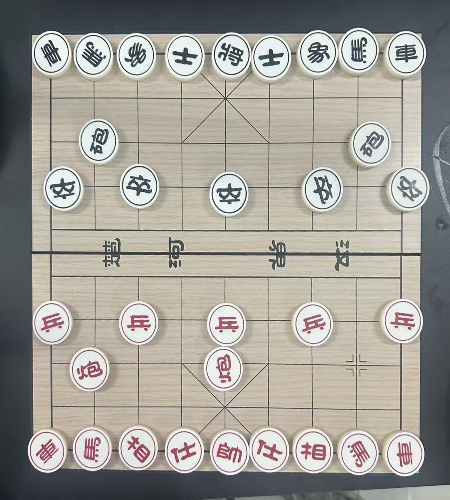
\includegraphics[width=0.55\textwidth]{figures/board_top.jpg}
\caption{系统采集的真实棋盘图像示例（调试用）。经 RTMPose 四角定位与透视校正后送入全局分类器。}
\label{fig:photo}
\end{figure}

% ============================================================
\chapter{棋局决策引擎与棋局表示}
\label{ch:ai}

\section{Pikafish 与 UCI 协议}
\label{sec:uci}
认知层通过 UCI 协议驱动 Pikafish 引擎\cite{pikafish2024,uci2004}。\texttt{AIEngine} 的启动序列为：
发送 \texttt{uci} 并等待 \texttt{uciok}；设置 \texttt{UCI\_Variant value xiangqi} 以启用中国象棋变体；
设置 \texttt{Skill Level}（取自 \texttt{ENGINE\_DEPTH}=15）与可选的 \texttt{Hash}（\texttt{HASH\_SIZE\_MB}=128）。
决策时，引擎以 \texttt{position fen <FEN> [moves ...]} 载入局面，再以 \texttt{go depth 15} 搜索，
解析 stdout 中的 \texttt{bestmove} 作为推荐着法；\texttt{analyze\_position} 则改用 \texttt{go movetime}
并解析 \texttt{info ... score cp/depth/pv} 以呈现评分与主要变化。默认引擎二进制为
\texttt{Pikafish/pikafish-avx2.exe}，配套 NNUE 权重约 $50.8$~MiB。

\section{搜索引擎原理}
\label{sec:search}
现代棋类引擎的搜索以\textbf{极小化极大（minimax）}框架为基础：在博弈树上交替最大化己方、最小化
对方收益。为在有限时间内深入搜索，引擎普遍采用以下技术\cite{russell2020ai}：
\begin{itemize}[itemsep=2pt]
  \item \textbf{alpha-beta 剪枝}：在遍历博弈树时维护 $\alpha$（己方已可保证的下界）与 $\beta$
        （对方已可保证的上界），一旦区间为空即剪掉该子树，可将有效分支因子由 $b^d$ 降至约 $b^{d/2}$。
  \item \textbf{迭代加深（iterative deepening）}：从浅层逐步加深搜索深度，既保证随时可返回最佳着法，
        又能以浅层结果排序引导深层移动顺序、提升剪枝效率。
  \item \textbf{静态搜索（quiescence search）}：在叶子节点继续搜索吃子等“不稳定”着法，抑制
        水平效应（horizon effect）带来的评估抖动。
  \item \textbf{NNUE 神经评估}：以增量更新的半接（half-KP）特征配合小型神经网络评估局面，取代
        手工评估函数，显著提升棋力\cite{nasu2018nnue}。本系统 NNUE 权重约 $50.8$~MiB，由引擎在
        启动时载入。
\end{itemize}

\section{中国象棋 FEN 与坐标表示}
\label{sec:fen}
系统采用扩展 FEN 表示棋局，开局串为
\begin{quote}
\texttt{rnbakabnr/9/1c5c1/p1p1p1p1p/9/9/P1P1P1P1P/1C5C1/9/RNBAKABNR w - - 0 1}
\end{quote}
棋盘为 $10$ 行 $\times$ $9$ 列，每方 $7$ 类棋子（车/马/相(象)/士(仕)/帅(将)/炮/兵(卒)）。FEN 的首行
对应棋盘第 9 行（黑方底线），末行对应第 0 行（红方底线）；走子方用 \texttt{w}/\texttt{b} 表示，本系统中
\texttt{w} 代表红方先行\cite{xqfen2007}。\texttt{FENUtils} 提供 \texttt{parse\_fen}、\texttt{to\_fen} 与
\texttt{extract\_move\_from\_fen\_change}（通过对比前后两局 FEN 还原一步 UCI 着法），是连接视觉识别与
决策的核心数据契约。棋子字符与基础属性如表~\ref{tab:fen} 所示。

\begin{table}[H]
\centering
\caption{中国象棋 FEN 棋子字符与基础属性}
\label{tab:fen}
\renewcommand{\arraystretch}{1.2}
\begin{tabular}{@{}lccccccc@{}}
\toprule
 & 车 & 马 & 相/象 & 士/仕 & 帅/将 & 炮 & 兵/卒 \\
\midrule
红方 & \texttt{R} & \texttt{N} & \texttt{B} & \texttt{A} & \texttt{K} & \texttt{C} & \texttt{P} \\
黑方 & \texttt{r} & \texttt{n} & \texttt{b} & \texttt{a} & \texttt{k} & \texttt{c} & \texttt{p} \\
棋盘 & \multicolumn{7}{c}{$9$ 列 $\times$ $10$ 行，含河界与九宫} \\
\bottomrule
\end{tabular}
\end{table}

\section{着法记谱转换}
为便于人机界面展示，\texttt{MoveNotationUtils} 在 UCI 坐标记法（如 \texttt{h2e2}）与中文/简易 WXF
记法间互转。UCI 以“起点列行 + 终点列行”编码；中文记法则以“棋子名 + 起点路数/线数 + 进退/平 + 终点”
表达（如“炮二平五”），二者通过 \texttt{xq\_utils/coordinates.py} 中的列行索引换算衔接。

% ============================================================
\chapter{机械臂控制与通信协议}
\label{ch:robot}

\section{五值 ASCII 指令协议}
\label{sec:proto}
执行层定义了一种极简的\textbf{五值指令协议}：上位机每步仅下发五个以逗号分隔的整数
\begin{quote}
\texttt{startX, startY, endX, endY, signal}
\end{quote}
其中 \texttt{signal}=0 表示普通移动，\texttt{signal}=1 表示吃子（抓取目标位已有棋子）。所有角度解算
与气泵时序均在 STM32 下位机侧完成。该协议经 \textbf{TCP 端口 8086} 下发，默认主机为
\texttt{192.168.0.102}。协议字段语义如表~\ref{tab:proto} 所示。极小的协议表面积使上位机逻辑简单、
易于测试（协议测试直接断言几何与 ACK）。

\begin{table}[H]
\centering
\caption{五值指令协议字段语义}
\label{tab:proto}
\renewcommand{\arraystretch}{1.25}
\begin{tabularx}{\textwidth}{@{}>{\ttfamily\small}l X@{}}
\toprule
字段 & 含义 \\
\midrule
startX, startY & 起点在机械臂坐标系下的 $x,y$（毫米） \\
endX, endY & 终点在机械臂坐标系下的 $x,y$（毫米） \\
signal & 0=普通移动；1=吃子（需先移走被吃子） \\
帧格式 & 以 \textbackslash r\textbackslash n（CRLF）结尾；归位指令为 \texttt{-17.1848,-55.6304,0,0,99} \\
完成确认 & 下位机回复含 \texttt{STATE:5} 且 \texttt{RESULT:1} 的报文表示动作完成 \\
\bottomrule
\end{tabularx}
\end{table}

\section{棋盘坐标到机械臂坐标的映射}
\label{sec:mapping}
机械臂坐标系以棋盘\textbf{右上角交叉点}（黑方右车位）为原点。设第 $f$ 列（$0\le f\le 8$）、
第 $r$ 行（$0\le r\le 9$，$r=9$ 为黑方底线）的交叉点到原点的映射为
\begin{equation}
\label{eq:map}
\begin{aligned}
x &= x_0 + (8 - f)\times s_f, \\
y &= y_0 + (9 - r)\times s_r + \delta_r, \\
\delta_r &= \begin{cases}
s_{\text{river}} - s_r, & r \le 4 \quad\text{（红方半场，叠加河界间隔）}\\
0, & r > 4
\end{cases}
\end{aligned}
\end{equation}
其中列间距 $s_f=34$~mm、普通行间距 $s_r=30$~mm、河界行间距 $s_{\text{river}}=32$~mm。由此可得棋盘
总宽 $34\times 8 = 272$~mm、总高 $30\times 8 + 32 = 272$~mm，即 $272\times272$~mm 的正方形盘面
（图~\ref{fig:geom}）。该几何与固件文档的测量值一致，是上位机与下位机对齐的物理基础。

\begin{figure}[H]
\centering
\adjustbox{max width=0.7\textwidth}{%
\begin{tikzpicture}[font=\small]
  \def\stepc{1.15}
  \pgfmathsetmacro{\gw}{8*\stepc}
  \pgfmathsetmacro{\gh}{9*\stepc}
  \draw[step=\stepc cm, thin, gray!60] (0,0) grid (\gw,\gh);
  \draw[thick, blue!70!black, dashed] (0,5*\stepc) -- (\gw,5*\stepc)
        node[midway, above, font=\tiny, blue!70!black] {河界 (river, 32\,mm)};
  \fill[red] (\gw,\gh) circle (3pt) node[above right, font=\tiny, red] {原点 (黑方右车)};
  \draw[<->] (\gw, \gh+0.5) -- (\gw-\stepc, \gh+0.5) node[midway, above, font=\tiny] {$34$\,mm};
  \draw[<->] (\gw+0.5, \gh) -- (\gw+0.5, \gh-\stepc) node[midway, right, font=\tiny] {$30$\,mm};
  \node at (\gw/2, -0.7) [font=\tiny, gray] {$9$ 列 $\times$ $10$ 行，总尺寸 $272\times272$\,mm};
\end{tikzpicture}}
\caption{棋盘几何与坐标映射示意。原点位于右上角（黑方右车），列间距 34\,mm、普通行间距 30\,mm、
河界行间距 32\,mm。}
\label{fig:geom}
\end{figure}

\section{持久化 TCP 客户端与确认握手}
\label{sec:handshake}
\texttt{RobotPersistentClient} 以 \texttt{socket.create\_connection} 建立长连接，并设置
\texttt{SO\_KEEPALIVE} 与 \texttt{TCP\_NODELAY}。每条指令以 CRLF 成帧；\texttt{send\_robot\_command}
阻塞直至收到 \texttt{motion\_acknowledged}（要求响应同时含 \texttt{STATE:5} 与 \texttt{RESULT:1}），
由于运动指令非幂等，客户端在缺失 ACK 时\textbf{不自动重发}而直接报错。归位指令
\texttt{send\_homing\_command} 发送 \texttt{-17.1848, -55.6304, 0, 0, 99}（命令号 99 标记归位），
并等待 \texttt{homing\_acknowledged}。Web 端在硬件模式下启动对局前必须先完成归位握手，否则以
HTTP 503 拒绝开局。\texttt{UCI\_Variant=xiangqi} 的 Pikafish 使用 $0$--$9$ 的行列编号，因此
\texttt{uci\_to\_arm\_command} 直接按该约定解析并调用式~(\ref{eq:map}) 完成映射。

上位机与 STM32 之间的典型交互时序如图~\ref{fig:seq} 所示。

\begin{figure}[H]
\centering
\adjustbox{max width=0.6\textwidth}{%
\begin{tikzpicture}[font=\small, >=Latex, scale=0.9]
  \draw[->] (0,0) -- (0,-8) node[below] {上位机 (Host)};
  \draw[->] (6,0) -- (6,-8) node[below] {STM32 下位机};
  \draw[->,thick] (0,-0.6) -- node[above,font=\tiny,align=center] {TCP connect\\(端口 8086)} (6,-0.6);
  \draw[->,thick] (0,-1.8) -- node[above,font=\tiny,align=center] {homing 指令\\(-17.18,-55.63,0,0,99)} (6,-1.8);
  \draw[<-,thick] (0,-3.0) -- node[above,font=\tiny,align=center] {STATE:5\\RESULT:1} (6,-3.0);
  \draw[->,thick] (0,-4.2) -- node[above,font=\tiny,align=center] {move 指令\\(sx,sy,ex,ey,sig)} (6,-4.2);
  \draw[<-,thick] (0,-5.4) -- node[above,font=\tiny,align=center] {STATE:5\\RESULT:1} (6,-5.4);
  \draw[->,thick,dotted] (0,-6.6) -- node[above,font=\tiny] {重复 move + ACK} (6,-6.6);
\end{tikzpicture}}
\caption{上位机与 STM32 的通信时序：连接后先归位握手，再逐条下发五值移子指令并等待完成确认。}
\label{fig:seq}
\end{figure}

\section{STM32 下位机实现与运动学}
\label{sec:firmware}
激活的固件 \texttt{firmware/stm32-f103-angle-plan} 在 STM32F103 上以 \texttt{sscanf} 解析
五整数格式的指令串 \texttt{"\%d, \%d, \%d, \%d, \%d"}，于片内完成运动学解算与气泵抓取时序\cite{stm32f103}。
以平面 SCARA 型机械臂为例，其正向运动学为
\begin{equation}
\label{eq:fk}
\begin{aligned}
x &= L_1\cos\theta_1 + L_2\cos(\theta_1+\theta_2), \\
y &= L_1\sin\theta_1 + L_2\sin(\theta_1+\theta_2),
\end{aligned}
\end{equation}
下位机依据目标 $(x,y)$ 反解关节角 $(\theta_1,\theta_2)$ 后，由定时器输出 PWM 驱动步进/伺服电机，
并以 GPIO 控制气泵电磁阀完成“吸起—平移—放下”的移子动作\cite{craig2017robotics}。系统中另保留一个
\textbf{已弃用}的 JSON 传输栈（\texttt{robot/legacy\_tcp\_client.py} 经 TCP 端口 5000 下发 JSON，
配套 \texttt{firmware/stm32-tcp-server}），它不再被主程序使用，仅作为历史固件的兼容客户端保留。
论文明确区分二者，以免混淆激活路径。

% ============================================================
\chapter{软件编排与 Web 仿真}
\label{ch:web}

\section{Flask 组合根与蓝图架构}
\label{sec:flask}
\texttt{web\_simulation} 是系统的激活控制路径，以 Flask 在端口 5000 提供服务\cite{flask2024}。
\texttt{app.py} 作为组合根，持有可变的共享 \texttt{game\_state} 字典与若干长生命周期组件（识别器、引擎、
机器人控制器、TCP 客户端），并通过蓝图将路由拆分为 \texttt{status}、\texttt{camera}、
\texttt{recognition} 与 \texttt{game} 四个职责域。纯棋局函数集中在 \texttt{domain.py}
（如 \texttt{board\_state\_to\_fen}、\texttt{apply\_uci\_to\_board\_state}），机器人指令封装在
\texttt{robot\_cmd.py}，状态机与硬件/仿真切换在 \texttt{game\_logic.py}。该结构使 Web 层与核心算法
解耦，便于在无浏览器环境下以单元测试覆盖领域逻辑。

\section{双模式对弈与人机交互}
\label{sec:dual}
系统支持\textbf{硬件}与\textbf{仿真}两种机器人模式（默认硬件）。硬件模式下，\texttt{apply\_ai\_best\_move}
将 AI 走法转换为五值指令、预应用到棋盘状态、暂停视觉、下发至 STM32 并等待 \texttt{STATE:5,RESULT:1}；
仿真模式则在本地模拟走子。Web 界面（\texttt{templates/index.html} + \texttt{static/js/app.js}）提供：
实时摄像头 MJPEG 流与本地/网络摄像头切换、单步与连续棋盘识别、开局（硬件先归位）、AI 走子与
实时评分（depth/score/pv/nodes）、手动或自动识别玩家走子，以及 FEN、棋局状态、走子历史、回合、
机器人状态与连接探测等可视化。

% ============================================================
\chapter{工程实现与质量保障}
\label{ch:eng}

\section{代码规模与解耦}
\label{sec:scale}
重构后的系统以“纯函数包 + 职责包 + 组合根”组织，便于单元测试与替换。各包的代码规模如表~\ref{tab:scale}
所示（不含注释与空行，固件为 C/C++ 源）。整库约 $6\,500$ 行 Python 与 $6\,400$ 行固件代码。

\begin{table}[H]
\centering
\caption{主要模块代码规模（实测）}
\label{tab:scale}
\renewcommand{\arraystretch}{1.2}
\begin{tabular}{@{}lrr@{}}
\toprule
模块 & Python 文件数 & 代码行数（不含注释/空行） \\
\midrule
\texttt{xq\_utils} & 5 & 448 \\
\texttt{cli} & 3 & 261 \\
\texttt{game\_manager} & 4 & 445 \\
\texttt{vision} & 9 & 1\,397 \\
\texttt{ai} & 2 & 324 \\
\texttt{robot} & 4 & 921 \\
\texttt{core} & 7 & 821 \\
\texttt{web\_simulation} & 12 & 1\,933 \\
\texttt{config.py} & 1 & 115 \\
\midrule
\textbf{小计（Python）} & \textbf{47} & \textbf{约 6\,665} \\
\textbf{firmware（C/C++）} & 27 & 6\,448 \\
\bottomrule
\end{tabular}
\end{table}

\section{测试体系}
\label{sec:tests}
系统在 \texttt{tests/} 下提供 $10$ 个测试模块、共 $76$ 个测试方法，覆盖摄像头与图像来源、稳定器与
识别并发、五值协议与 Web 后端循环、前端归位契约、STM32 归位契约与 Web 领域函数等。最近一次运行
结果为 $75$ 项通过、$1$ 项未通过——该失败源于运行环境的一个特定限制（某 Windows 环境变量超过
$32\,767$ 字符导致 \texttt{mock.patch.dict} 异常），与识别/协议逻辑无关。协议与后端循环测试
（约占全部测试方法的一半）直接断言了五值几何（实测 34/30/32\,mm）、吃子信号、归位共享客户端与
“无自动重发”等关键不变量。

\section{ONNX 推理与执行提供者}
\label{sec:onnx}
\begin{sloppypar}
\texttt{core/\allowbreak runonnx} 的推理后端按优先级选择 \texttt{CUDAExecutionProvider} →
\texttt{DmlExecutionProvider} → \texttt{CPUExecutionProvider}，在缺失 CUDA~12 / cuDNN~9 运行库时
自动回退至 CPU，并启用 \texttt{ORT\_ENABLE\_ALL} 图优化，保证在无 GPU 环境下仍可运行（仅推理速度下降）\cite{onnxruntime2024}。
\end{sloppypar}

% ============================================================
\chapter{实验与系统指标}
\label{ch:exp}
本节汇总可在代码仓库中\textbf{直接核验}的系统指标。我们刻意避免给出未经真实硬件测量的精度或
时延数字，以保证结论的可复现性；涉及性能的下界/上界以“设计特征”或“规格参数”明确标注。

模型规格方面，两个默认 ONNX 模型与 NNUE 权重的体积与张量形状如表~\ref{tab:models} 所示，均为
仓库内真实文件。配置常量方面，表~\ref{tab:config} 列出与识别、决策、控制相关的关键参数（取自
\texttt{config.py}）。

\begin{table}[H]
\centering
\caption{模型与权重规格（仓库真实文件）}
\label{tab:models}
\renewcommand{\arraystretch}{1.2}
\begin{tabularx}{\textwidth}{@{}>{\ttfamily\small}l >{\small}l r >{\small}X >{\small}X@{}}
\toprule
文件 & 角色 & 大小 & 输入 & 输出 \\
\midrule
4\_v6-0301.onnx & RTMPose 四角关键点 & $\approx$10.2\,MiB & $256\times256$ & SimCC $4\times512$（x,y） \\
nano\_v3-0319.onnx & 全局棋盘分类器 & $\approx$29.7\,MiB & $280\times315$ & $90\times16$ \\
pikafish.nnue & NNUE 评估权重 & $\approx$50.8\,MiB & — & — \\
\bottomrule
\end{tabularx}
\end{table}

\begin{table}[H]
\centering
\caption{关键配置常量（取自 \texttt{config.py}）}
\label{tab:config}
\renewcommand{\arraystretch}{1.2}
\begin{tabular}{@{}ll@{}}
\toprule
常量 & 取值 \\
\midrule
摄像头 & \texttt{CAMERA\_WIDTH}=640, \texttt{CAMERA\_HEIGHT}=480, \texttt{CAMERA\_FPS}=30 \\
棋盘 & \texttt{BOARD\_ROWS}=10, \texttt{BOARD\_COLS}=9 \\
稳定 & \texttt{STABLE\_WINDOW}=5, \texttt{STABLE\_RATIO}=0.60, \texttt{AUTO\_STABLE\_FRAMES}=25 \\
引擎 & \texttt{ENGINE\_DEPTH}=15, \texttt{THINK\_TIME}=5000\,ms, \texttt{HASH\_SIZE\_MB}=128 \\
机器人网络 & \texttt{ROBOT\_NETWORK\_PORT}=8086, \texttt{ROBOT\_NETWORK\_HOST}=192.168.0.102 \\
机械臂几何 & $s_f$=34\,mm, $s_r$=30\,mm, $s_{\text{river}}$=32\,mm, 原点右上角 \\
归位 & \texttt{ROBOT\_HOMING\_M1}=-17.1848$^\circ$, \texttt{ROBOT\_HOMING\_M2}=-55.6304$^\circ$ \\
\bottomrule
\end{tabular}
\end{table}

% ============================================================
\chapter{讨论}
\label{ch:disc}

\section{设计权衡}
\label{sec:tradeoff}
系统在“识别精度”与“推理开销”之间选择了整盘一次性分类而非逐格/检测器方案，换取了边缘部署下的低
延迟与简单后处理；以四角关键点而非全棋盘角点检测做定位，则降低了对棋盘纹理完整性的依赖。在通信上，
五值 ASCII 协议刻意保持极小表面积，把运动学复杂性下沉到 STM32，使上位机逻辑简单且易于测试
（测试直接断言几何与 ACK）。

\section{已知不一致与可复现性说明}
\label{sec:inconsist}
论文必须如实指出代码库中存在两处坐标/几何约定差异，供后续维护者注意：
\begin{itemize}[itemsep=2pt]
  \item \texttt{xq\_utils/coordinates.py} 采用 $1$--$10$ 的行列编号与 $50$~mm 方格（左上角原点），
        服务于仿真控制器；而激活的硬件路径（\texttt{robot/protocol.py} 与 \texttt{web\_simulation/domain.py}）
        采用 $0$--$9$ 编号与实测 34/30/32\,mm 几何（右上角原点），以匹配 Pikafish 的 UCI 变体与固件。
        二者暂无显式适配层，属于历史演进遗留，建议在重构时统一。
  \item 存在激活的五值 8086 传输栈与已弃用的 JSON 5000 传输栈并存，主程序仅使用前者。
\end{itemize}
此外，\texttt{config.py} 中仍保留若干针对早期 YOLO 方案的配置项（如 \texttt{YOLO\_MODEL\_PATH}），
当前识别流水线已不加载该类模型，属历史残留，建议清理以免误导。

\section{局限性}
\label{sec:limit}
本文的实验部分仅给出可在仓库核验的规格与测试覆盖，未包含真实硬件下的识别准确率、单步移子时延与
长时间运行稳定性等经验指标——这需要实体机械臂与标定环境，留作后续工作。

% ============================================================
\chapter{结论与展望}
\label{ch:conc}
本文介绍了 CH-RO 中国象棋对弈机器人系统，覆盖从视觉棋盘识别、Pikafish UCI 决策到 STM32 五值
指令执行的完整闭环，并以 Flask Web 界面贯通人机交互。系统通过 RTMPose 四角关键点 + 全局分类器的
轻量识别方案、确定性的五值指令与完成确认握手，以及硬件/仿真双模式，在解耦、可测试的代码架构下
实现了端到端对弈。

未来工作包括：(1) 统一坐标与几何约定，消除仿真/硬件路径差异；(2) 在真实硬件上建立识别准确率与
移子时延的基准评测；(3) 引入更轻量的分类/关键点模型以提升边缘实时性；(4) 扩展开局库、残局表与
更强的时限/难度控制，丰富对弈体验。

% ============================================================
\printbibliography[title=参考文献]

\end{document}
